\documentclass[border=3mm]{standalone}
\usepackage{tikz}
\usetikzlibrary{arrows.meta,positioning,shapes.geometric,shapes.misc,fit,calc,backgrounds,decorations.pathreplacing}
\usepackage{amsmath,amssymb}

% Publication-grade palette matching main methodology
\definecolor{colRisk}{HTML}{922B21}   % Deep Crimson: Security Risk Features
\definecolor{colThreat}{HTML}{B9770E} % Amber Ochre: Threat Severity & Adversary
\definecolor{colRes}{HTML}{1A5276}    % Slate Blue: Infrastructure Telemetry
\definecolor{colQoS}{HTML}{1E8449}    % Forest Green: Availability & QoS
\definecolor{colDRL}{HTML}{0E6655}    % Deep Teal: Latent & Policy Heads
\definecolor{gatecol}{HTML}{D35400}   % Gating Accent

\begin{document}
\sffamily\footnotesize
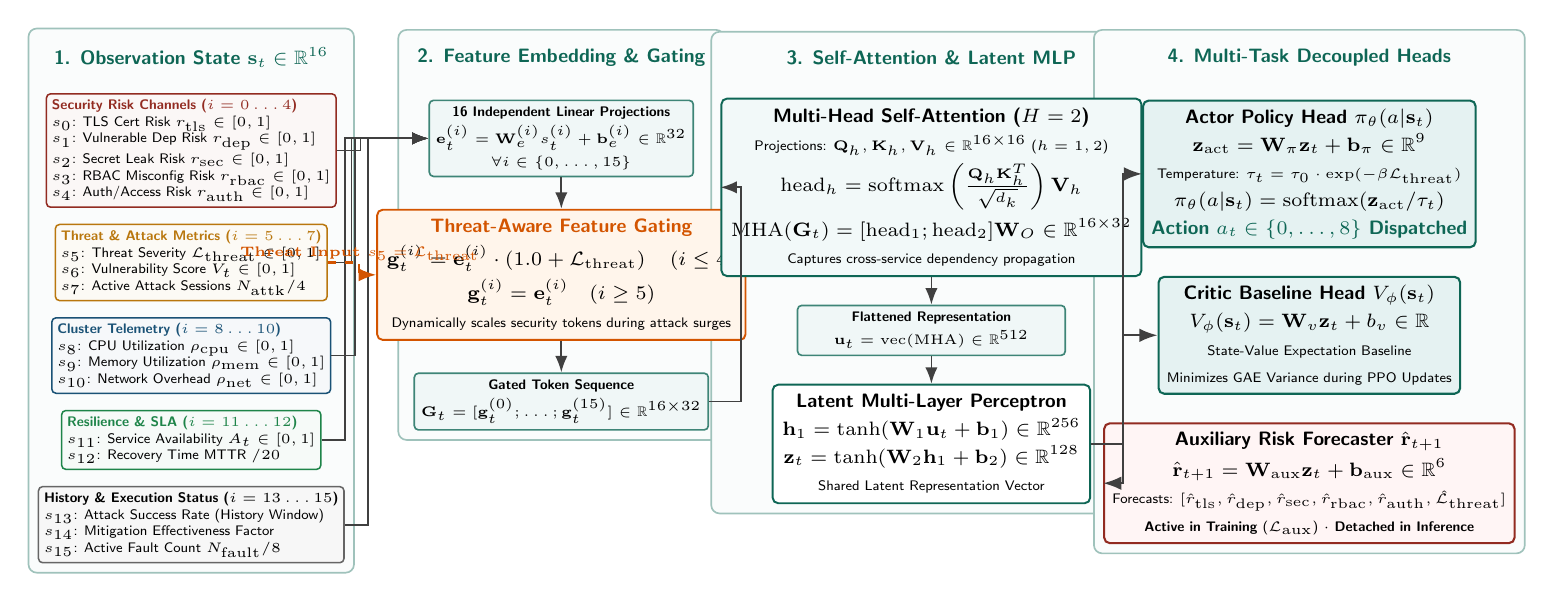
\begin{tikzpicture}[
    >=Latex,
    font=\sffamily,
    featbox/.style={
        draw=black!70, line width=0.55pt, fill=white,
        rounded corners=1.5pt, inner sep=2pt, align=left,
        font=\sffamily\tiny, minimum width=32mm
    },
    embbox/.style={
        draw=colDRL!80, line width=0.6pt, fill=teal!6,
        rounded corners=1.5pt, inner sep=2.5pt, align=center,
        font=\sffamily\tiny, minimum width=22mm
    },
    procbox/.style={
        draw=colDRL, line width=0.7pt, fill=white,
        rounded corners=2pt, inner sep=3.5pt, align=center,
        font=\sffamily\scriptsize
    },
    headbox/.style={
        draw=colDRL, line width=0.75pt, fill=teal!10,
        rounded corners=2pt, inner sep=3pt, align=center,
        font=\sffamily\scriptsize
    },
    secflow/.style={
        ->, line width=0.65pt, draw=black!75
    },
    gateflow/.style={
        ->, dashed, line width=0.75pt, draw=gatecol
    }
]

% ==============================================================================
% STAGE 1: 16-DIMENSIONAL OBSERVATION VECTOR (INPUTS)
% ==============================================================================
\node[font=\sffamily\bfseries\scriptsize, text=colDRL] (hdr_input) at (0, 7.8) {1. Observation State $\mathbf{s}_t \in \mathbb{R}^{16}$};

% Category 1: Security Risks (s0 - s4)
\node[featbox, draw=colRisk, fill=colRisk!4, below=2mm of hdr_input] (f_risks) {
    \textbf{\textcolor{colRisk}{Security Risk Channels ($i=0\dots4$)}}\\
    $s_0$: TLS Cert Risk $r_{\mathrm{tls}} \in [0, 1]$\\
    $s_1$: Vulnerable Dep Risk $r_{\mathrm{dep}} \in [0, 1]$\\
    $s_2$: Secret Leak Risk $r_{\mathrm{sec}} \in [0, 1]$\\
    $s_3$: RBAC Misconfig Risk $r_{\mathrm{rbac}} \in [0, 1]$\\
    $s_4$: Auth/Access Risk $r_{\mathrm{auth}} \in [0, 1]$
};

% Category 2: Threat & Adversary (s5 - s7)
\node[featbox, draw=colThreat, fill=colThreat!4, below=2mm of f_risks] (f_threat) {
    \textbf{\textcolor{colThreat}{Threat \& Attack Metrics ($i=5\dots7$)}}\\
    $s_5$: Threat Severity $\mathcal{L}_{\mathrm{threat}} \in [0, 1]$\\
    $s_6$: Vulnerability Score $V_t \in [0, 1]$\\
    $s_7$: Active Attack Sessions $N_{\mathrm{attk}} / 4$
};

% Category 3: Cluster Resources (s8 - s10)
\node[featbox, draw=colRes, fill=colRes!4, below=2mm of f_threat] (f_res) {
    \textbf{\textcolor{colRes}{Cluster Telemetry ($i=8\dots10$)}}\\
    $s_8$: CPU Utilization $\rho_{\mathrm{cpu}} \in [0, 1]$\\
    $s_9$: Memory Utilization $\rho_{\mathrm{mem}} \in [0, 1]$\\
    $s_{10}$: Network Overhead $\rho_{\mathrm{net}} \in [0, 1]$
};

% Category 4: Availability & QoS (s11 - s12)
\node[featbox, draw=colQoS, fill=colQoS!4, below=2mm of f_res] (f_qos) {
    \textbf{\textcolor{colQoS}{Resilience \& SLA ($i=11\dots12$)}}\\
    $s_{11}$: Service Availability $A_t \in [0, 1]$\\
    $s_{12}$: Recovery Time MTTR $/ 20$
};

% Category 5: History & Faults (s13 - s15)
\node[featbox, draw=black!60, fill=black!3, below=2mm of f_qos] (f_hist) {
    \textbf{History \& Execution Status ($i=13\dots15$)}\\
    $s_{13}$: Attack Success Rate (History Window)\\
    $s_{14}$: Mitigation Effectiveness Factor\\
    $s_{15}$: Active Fault Count $N_{\mathrm{fault}} / 8$
};

% ==============================================================================
% STAGE 2: LINEAR FEATURE EMBEDDING & THREAT-AWARE GATING
% ==============================================================================
\node[font=\sffamily\bfseries\scriptsize, text=colDRL] (hdr_emb) at (4.7, 7.8) {2. Feature Embedding \& Gating};

% Feature Projection Block
\node[embbox, below=3mm of hdr_emb, minimum width=30mm] (proj_block) {
    \textbf{16 Independent Linear Projections}\\[1pt]
    $\mathbf{e}_t^{(i)} = \mathbf{W}_e^{(i)} s_t^{(i)} + \mathbf{b}_e^{(i)} \in \mathbb{R}^{32}$\\[1pt]
    $\forall i \in \{0, \dots, 15\}$
};

% Gating Multiplier Unit
\node[procbox, draw=gatecol, fill=orange!8, below=4mm of proj_block, minimum width=30mm] (gating_unit) {
    \textbf{\textcolor{gatecol}{Threat-Aware Feature Gating}}\\[2pt]
    $\mathbf{g}_t^{(i)} = \mathbf{e}_t^{(i)} \cdot \left(1.0 + \mathcal{L}_{\mathrm{threat}}\right) \quad (i \le 4)$\\[2pt]
    $\mathbf{g}_t^{(i)} = \mathbf{e}_t^{(i)} \quad (i \ge 5)$\\[2pt]
    \tiny Dynamically scales security tokens during attack surges
};

% Token Stack Representation
\node[embbox, below=4mm of gating_unit, minimum width=30mm] (token_stack) {
    \textbf{Gated Token Sequence}\\[1pt]
    $\mathbf{G}_t = [\mathbf{g}_t^{(0)}; \dots; \mathbf{g}_t^{(15)}] \in \mathbb{R}^{16 \times 32}$
};

% Connections from Inputs to Embedding & Gating
\draw[secflow] (f_risks.east) -- ++(0.3,0) |- (proj_block.west);
\draw[secflow] (f_threat.east) -- ++(0.3,0) |- (proj_block.west);
\draw[secflow] (f_res.east) -- ++(0.3,0) |- (proj_block.west);
\draw[secflow] (f_qos.east) -- ++(0.3,0) |- (proj_block.west);
\draw[secflow] (f_hist.east) -- ++(0.3,0) |- (proj_block.west);

\draw[secflow] (proj_block) -- (gating_unit);
% Threat severity modulation line
\draw[gateflow] (f_threat.east) -- ++(0.4, 0) |- (gating_unit.west)
    node[pos=0.35, above, font=\tiny\bfseries, text=gatecol] {Threat Input $s_5 = \mathcal{L}_{\mathrm{threat}}$};
\draw[secflow] (gating_unit) -- (token_stack);

% ==============================================================================
% STAGE 3: MULTI-HEAD SELF-ATTENTION & LATENT ENCODER
% ==============================================================================
\node[font=\sffamily\bfseries\scriptsize, text=colDRL] (hdr_attn) at (9.4, 7.8) {3. Self-Attention \& Latent MLP};

% MHSA Block
\node[procbox, draw=colDRL, fill=teal!5, below=3mm of hdr_attn, minimum width=34mm] (mhsa_unit) {
    \textbf{Multi-Head Self-Attention ($H=2$)}\\[2pt]
    \tiny Projections: $\mathbf{Q}_h, \mathbf{K}_h, \mathbf{V}_h \in \mathbb{R}^{16 \times 16}$ ($h=1,2$)\\[2pt]
    $\mathrm{head}_h = \mathrm{softmax}\left(\frac{\mathbf{Q}_h \mathbf{K}_h^T}{\sqrt{d_k}}\right) \mathbf{V}_h$\\[2pt]
    $\mathrm{MHA}(\mathbf{G}_t) = [\mathrm{head}_1; \mathrm{head}_2]\mathbf{W}_O \in \mathbb{R}^{16 \times 32}$\\[2pt]
    \tiny Captures cross-service dependency propagation
};

% Flattening Node
\node[embbox, below=3.5mm of mhsa_unit, minimum width=34mm] (flatten_node) {
    \textbf{Flattened Representation}\\[1pt]
    $\mathbf{u}_t = \mathrm{vec}(\mathrm{MHA}) \in \mathbb{R}^{512}$
};

% Latent Dense MLP
\node[procbox, draw=colDRL, fill=white, below=3.5mm of flatten_node, minimum width=34mm] (dense_mlp) {
    \textbf{Latent Multi-Layer Perceptron}\\[2pt]
    $\mathbf{h}_1 = \tanh(\mathbf{W}_1 \mathbf{u}_t + \mathbf{b}_1) \in \mathbb{R}^{256}$\\[2pt]
    $\mathbf{z}_t = \tanh(\mathbf{W}_2 \mathbf{h}_1 + \mathbf{b}_2) \in \mathbb{R}^{128}$\\[2pt]
    \tiny Shared Latent Representation Vector
};

\draw[secflow] (token_stack.east) -- ++(0.4, 0) |- (mhsa_unit.west);
\draw[secflow] (mhsa_unit) -- (flatten_node);
\draw[secflow] (flatten_node) -- (dense_mlp);

% ==============================================================================
% STAGE 4: THREE DECOUPLED MULTI-TASK OUTPUT HEADS
% ==============================================================================
\node[font=\sffamily\bfseries\scriptsize, text=colDRL] (hdr_heads) at (14.2, 7.8) {4. Multi-Task Decoupled Heads};

% Head 1: Actor Policy
\node[headbox, below=3mm of hdr_heads, minimum width=38mm] (actor_head) {
    \textbf{Actor Policy Head $\pi_\theta(a|\mathbf{s}_t)$}\\[2pt]
    $\mathbf{z}_{\mathrm{act}} = \mathbf{W}_\pi \mathbf{z}_t + \mathbf{b}_\pi \in \mathbb{R}^9$\\[2pt]
    \tiny Temperature: $\tau_t = \tau_0 \cdot \exp(-\beta \mathcal{L}_{\mathrm{threat}})$\\[2pt]
    $\pi_\theta(a|\mathbf{s}_t) = \mathrm{softmax}(\mathbf{z}_{\mathrm{act}} / \tau_t)$\\[2pt]
    \textbf{\textcolor{colDRL}{Action $a_t \in \{0, \dots, 8\}$ Dispatched}}
};

% Head 2: Critic Value Baseline
\node[headbox, below=3.5mm of actor_head, minimum width=38mm] (critic_head) {
    \textbf{Critic Baseline Head $V_\phi(\mathbf{s}_t)$}\\[2pt]
    $V_\phi(\mathbf{s}_t) = \mathbf{W}_v \mathbf{z}_t + b_v \in \mathbb{R}$\\[2pt]
    \tiny State-Value Expectation Baseline\\[2pt]
    \tiny Minimizes GAE Variance during PPO Updates
};

% Head 3: Auxiliary Risk Predictor
\node[headbox, draw=colRisk, fill=red!4, below=3.5mm of critic_head, minimum width=38mm] (aux_head) {
    \textbf{Auxiliary Risk Forecaster $\hat{\mathbf{r}}_{t+1}$}\\[2pt]
    $\hat{\mathbf{r}}_{t+1} = \mathbf{W}_{\mathrm{aux}} \mathbf{z}_t + \mathbf{b}_{\mathrm{aux}} \in \mathbb{R}^6$\\[2pt]
    \tiny Forecasts: $[\hat{r}_{\mathrm{tls}}, \hat{r}_{\mathrm{dep}}, \hat{r}_{\mathrm{sec}}, \hat{r}_{\mathrm{rbac}}, \hat{r}_{\mathrm{auth}}, \hat{\mathcal{L}}_{\mathrm{threat}}]$\\[2pt]
    \tiny \textbf{Active in Training} ($\mathcal{L}_{\mathrm{aux}}$) $\cdot$ \textbf{Detached in Inference}
};

% Branches from Dense Latent z_t to the 3 Heads
\draw[secflow, line width=0.8pt] (dense_mlp.east) -- ++(0.4, 0) |- (actor_head.west);
\draw[secflow, line width=0.8pt] (dense_mlp.east) -- ++(0.4, 0) |- (critic_head.west);
\draw[secflow, line width=0.8pt] (dense_mlp.east) -- ++(0.4, 0) |- (aux_head.west);

% ==============================================================================
% BACKGROUND REGION FRAMES & ANNOTATIONS
% ==============================================================================
\begin{scope}[on background layer]
    \node[draw=colDRL!40, line width=0.6pt, fill=colDRL!2, rounded corners=3pt,
          fit=(hdr_input) (f_risks) (f_hist)] (box1) {};
    \node[draw=colDRL!40, line width=0.6pt, fill=colDRL!2, rounded corners=3pt,
          fit=(hdr_emb) (proj_block) (token_stack)] (box2) {};
    \node[draw=colDRL!40, line width=0.6pt, fill=colDRL!2, rounded corners=3pt,
          fit=(hdr_attn) (mhsa_unit) (dense_mlp)] (box3) {};
    \node[draw=colDRL!40, line width=0.6pt, fill=colDRL!2, rounded corners=3pt,
          fit=(hdr_heads) (actor_head) (aux_head)] (box4) {};
\end{scope}

\end{tikzpicture}
\end{document}
